\section{Research proposal}
\label{sec:research-proposal}

This research proposal aims to optimize the data parallelism process by automatically updating the chunk size during the execution of an algorithm.
The primary strategy during optimization is evaluating the algorithm's memory footprint and fitting the predicted memory usage with the current chunk size.

As seen in section~\ref{sec:related-work}, while there have been numerous studies on historical analysis of memory usage to predict resource requirements, they are mainly from the scheduler perspective.
There is a significant gap in research regarding predicting the memory usage of a single algorithm, primarily focusing on data parallelism optimization.

\subsection{Problem statement}
\label{subsec:problem-statement}

The Discovery~\footnote{\url{https://discovery.ic.unicamp.br/}} laboratory, located at \ac{UNICAMP}~\footnote{\url{https://ic.unicamp.br/}}, is working on a seismic analysis project with Petrobras~\footnote{\url{https://petrobras.com.br/}}.
This project relies heavily on machine learning and seismic operators for its computing graphs.
However, the input of these graphs is a massive seismic dataset that can contain terabytes of data.
Even supercomputers do not have enough memory to handle the computation on a single node.
Therefore, usually the execution is distributed by using data parallelism.

To facilitate this process, our laboratory implemented a framework called \ac{DASF}~\cite{dasf} that simplifies the development of data-parallel computing graphs using Dask~\cite{dask} under the hood.
\ac{DASF}~\cite{dasf} has an input parameter called \textbf{block\_size} that defines the size of each seismic block used during data parallelism.
However, setting this parameter can be challenging because it required finding the optimal relationship between it and the network overhead caused by it.

To illustrate this challenge, I present image~\ref{fig:block\_size} which contains three computing graphs receiving input data from a seismic dataset.
The first graph shows the input data as the entire dataset, which requires a significant amount of memory to execute.
The second graph divides the data into thousands of small parts, reducing the memory requirement but adding network overhead.
The third graph divides the data into a smaller number of parts, minimizing both network and memory requirements.

\begin{figure}[h]
\label{fig:block-size}
\caption{Block size impact on memory and network usage}
\resizebox{\textwidth}{!}{%
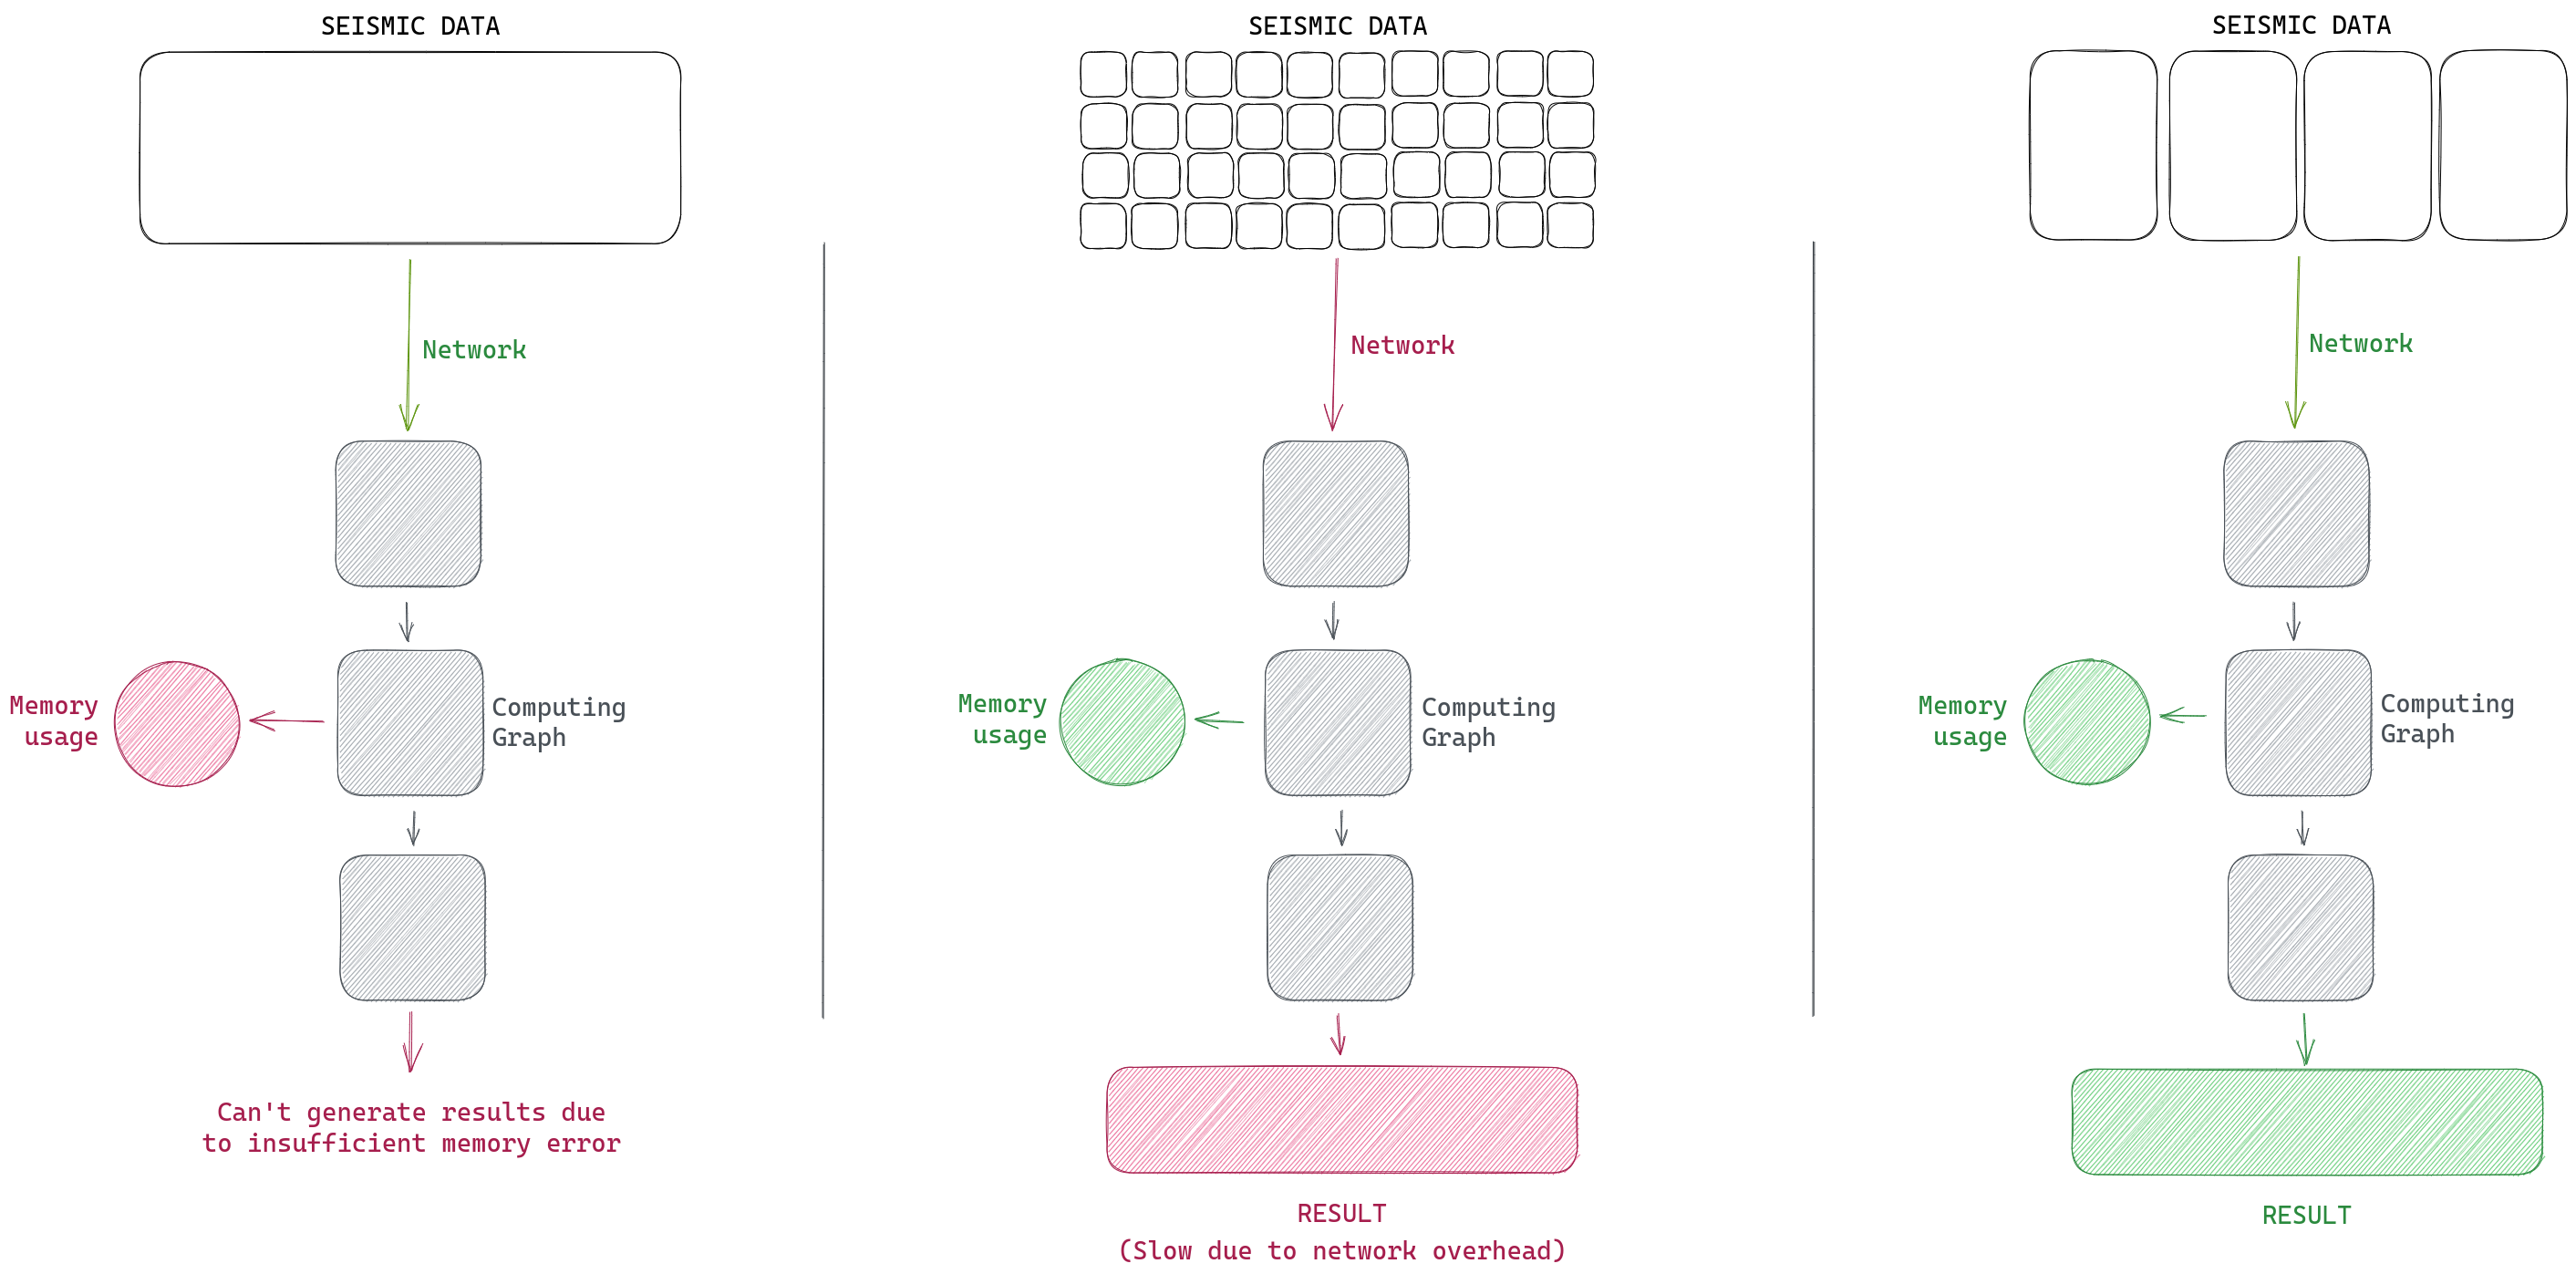
\includegraphics{block_size.png}
}
\end{figure}

While executing the graph, the developer must manually set the block\_size parameter.
Setting a large number may lead to memory issues and it causes a signifcant delay due the trial-and-error nature of the execution flow.
Since Petrobras uses supercomputers to execute those graphs, this delay is even larger considering the time it takes to submit a job due to the queue waiting time.

On the other hand, setting a small number may increase the execution time due to network overhead.
Since Petrobras have a large number of graphs to execute, and each graph usually takes a long time to execute, I need to find a way to optimize the block\_size parameter.

Dask~\cite{dask} provides an automatic chunking feature, but it relies on the chunk\_size parameter, which is a static parameter define prior to execution.
Since the developer do need to define this parameter prior to the execution, they can't rely on Dask~\cite{dask} auto chunking feature to automatically split the data, but they can rely on the automatic chunking if they figure out the ideal chunk\_size prior to the execution.

Figuring out the chunk\_size for algorithms that doesn't require a large working memory is easy, since the developer can set that to a percentagem of the available memory.
But, some of seismic operators used by Petrobras genereates a large working memory during the graph execution, which makes it difficult to determine the ideal chunk\_size.

Based on this assumption, if someone predicts the memory usage of the graph that person can use the Dask~\cite{dask} auto chunking feature to automatically split the data into the ideal number of chunks.
Since \ac{DASF}~\cite{dasf} uses Dask~\cite{dask} under the hood, the block\_size parameter on \ac{DASF}~\cite{dasf} is equivalent to the chunk\_size parameter on Dask~\cite{dask}.
Therefore, this research aims to develop an automated data partitioning strategy that is memory-footprint aware.
In other words, I aim to create a \ac{DASF}~\cite{dasf} plugin that can automatically set the optimal block\_size parameter during execution based on a machine learning model that can predict the memory-footprint of the algorithm.
This will help Petrobras to optimize resource utilization and minimize waiting and execution time.
The model will provide a comprehensive understanding of memory usage patterns for different block sizes and contribute to the development of a more efficient data partitioning strategy to execute a graph in large-scale clusters.

\subsection{Proposed solution}
\label{subsec:proposed-solution}

Most seismic operators are tensorial algorithms that execute calculations for each part of the input data.
Due to this fact, it is safe to assume that there might be a relationship between the memory usage of an algorithm and the shape of the input itself.
This research plans to create a reinforcement learning model that can optimize the chunking process by considering each task's memory footprint and adjusting the chunk size during the execution of the graph.

There are two different ways to implement the proposed solution:

\begin{enumerate}
  \item \textbf{Domain-specific model:} create a separate model for our domain, considering common input parameters, input shapes, and size as the primary features for the optimization;
  \item \textbf{Generic graph model:} create a single model capable of being graph-agnostic, considering the source code as a feature to describe the state during optimization.
\end{enumerate}

Although creating a generic model is more flexible, coding a domain-specific model will allow us to explore all possible limitations in a more controlled environment.
While coding the model, one of the first challenges is exploring which features may describe the current environment state for the optimization.
As a first hypothesis, the input data's shape and size may be the most relevant features since a large memory footprint is usually related to storing intermediate results.

Depending on the results of the initial experiments to create a domain-specific model, it is possible to expand the scope to a generic model.
In this scenario, all the tasks' source code within the graph may contain relevant information, such as how the code author deals with memory management.
However, it needs to be clarified how to extract features from the source code and use them to describe the current state during execution.

From a practical perspective, the reinforcement learning model will be responsible for the data partitioning process on \ac{DASF}~\cite{dasf}.
The goal is to create a plugin that can automatically decide the following action right after the execution of each task within the graph, allowing it to update to the optimal block size parameter during the execution of the graph.

\subsection{Potential risks and limitations}
\label{subsec:potential-risks-and-limitations}

In this section, I will discuss the limitations of the proposed solution for predicting memory consumption of seismic algorithms using machine learning.

\subsubsection{Sensibility towards too many control statements}

A possible limitation for this solution is that it may not work if the algorithm has too many control statements.
Depending on the structure of the algorithm, the amount of control statements may change the memory usage.

This limitation can be ignored if the memory allocation of the algorithm happens before the control statements.
On this scenario, even with control statements that change drastically the execution of the algorithm the memory usage will not change.

Either way, all the seismic operators and machine learning models being used are tensorial algorithms, which means that they do not have too many control statements.
Therefore, this possible limitation will not be a problem during the research.

\subsubsection{Unpredictable bottlenecks}

There are two possible memory bottlenecks in the proposed solution: CPU and GPU memory.
Seismic operators are likely to be GPU-memory bounded, but I need to conduct experiments to verify this.

If the algorithms can be both GPU-memory and CPU-memory bounded, then the proposed solution must be able to handle both scenarios.

\subsubsection{Language-agnosticit} y

The proposed solution is currently focused on using Python since it is the language used for the seismic operators and DASK~\cite{dask} itself.

Although Python is a popular language in the scientific community, it may not be the language of choice for all researchers.
This solution may not be language-agnostic at the moment.
However, in the future, I can improve the solution to accept algorithms from any language.

In the case of strategy one, presented on section ~\ref{subsubsec:algorithm-specific-model}, I can improve the training structure to accept algorithms from any language.
This can be done by allowing decoupling both the feature extraction, as well as the execution of the algorithm, from the training process.

In the case of strategy two, presented on section~\ref{subsubsec:generic-algorithm-model}, it is possible improve the feature-extraction part to allow more languages as well.
Since the only difference between the two strategies is allowing to exract features from the source code, a specialized feature extractor per-language should be enough.



\subsection{Problems to be addressed}
\label{subsec:problems-to-be-addressed}

In this section, I will outline the potential problems that I may encounter during our research and how I plan to address them.
Each problem is going to be presented as a subsection, with a brief description of the problem and how I plan to address it.

\subsubsection{How to measure memory usage}

One of the primary challenges in our research is accurately measuring memory usage.
This is particularly true for \ac{GPU} memory, which may differ from \ac{CPU} memory.
I aim to explore different options to measure memory usage accurately.

I plan to start by investigating if there is an API to measure \ac{GPU} memory, and if not, I will explore common libraries that allow gathering memory consumption based on a specific process.
I understand that the optimal approach would be to use a specific API for this, since this would allow more flexibility for our tool, but I will explore alternative options if necessary.

\subsubsection{Historical data requirements}

Many of the current approaches require a significant amount of historical data to train the models.
This is not feasible for our research, as it would be time-consuming to generate such data for algorithm-specific models.
I aim to overcome this limitation by creating a proper discovery approach by merging reinforcement learning with Bayesian analysis.

I plan to gather the minimal amount of data, even by executing the algorithm locally with a small amount of synthetic data, and then cover the exploration space for the input data for shapes and data with features the model have never seen before.
With this approach, I think the model will be able to learn while it is being used, and it will be able to generalize to new data.

\subsubsection{Python's garbage collection}

Python's garbage collector can pose a problem for us.
Python uses reference-counting as its garbage collection strategy, and it is lazy, so it usually waits for the memory to be needed to clean.
If our operators are \ac{CPU} memory bounded, I may need to figure out how to deal with Python's garbage collector to gather the real memory usage.
However, I will only need to address this issue depending on the results of our experiments.

\subsubsection{Graph execution}

Another problem I may encounter is how to figure out the entire graph's memory requirements.
While our proposed solution can help us find the amount of memory required for a specific algorithm, integrating multiple algorithms into a graph poses a challenge.
I plan to address this issue by predicting not only the memory usage, but alos the output shape of the algorithm and its features.
By having prior knowledge of the algorithms in the graph, I can compose a graph with the models using the output of the first model as the input data of the second one.

\subsection{Research questions and methodology}
\label{subsec:research-questions-and-methodology}

This section presents the research questions to explore in this study.
It also describes the methodology used to answer those questions.
Each research question is going to be answered by a set of experiments, grouped into three different categories, including:
(i) feasibility,
(ii) accuracy,
(iii) and applicability.
Table~\ref{tab:research-questions} summarizes the research questions and their categories.

\begin{table}[ht]
  \caption{Research questions}
  \label{tab:research-questions}
  \resizebox{\textwidth}{!}{%
    \begin{tabular}{@{}|l|l|l|@{} }
      \toprule
      \multicolumn{1}{|c|}{\textbf{\#}} & \textbf{Question}                                                            & \textbf{Category} \\ \midrule
      RQ1                               & How Dask~\cite{dask} deals with automatic chunking?                          & Feasibility       \\ \midrule
      RQ2                               & What is the optimal way of gathering memory-usage data?                      & Feasibility       \\ \midrule
      RQ3                               & Are seismic tensorial algorithms memory bounded by the \ac{CPU} or \ac{GPU}? & Feasibility       \\ \midrule
      RQ4                               & Which features do we need to extract from the input data?                    & Feasibility       \\ \midrule
      RQ5                               & What is the memory-usage behavior of our algorithms?                         & Accuracy          \\ \midrule
      RQ6                               & Under extreme circumstances, how is the memory usage of our algorithms?      & Accuracy          \\ \midrule
      RQ7                               & How to integrate the reinforcement learning model to execute chunking?        & Applicability     \\ \bottomrule
    \end{tabular}
  }
\end{table}

\subsubsection{Feasibility}
\label{subsubsec:feasibility-experiments}

This experiment category aims to answer \textbf{RQ1}, \textbf{RQ2}, \textbf{RQ3}, and \textbf{RQ4}.
The goal is to understand the feasibility of our seismic operators and their main characteristics.

This category will start with an experiment to explore how Dask~\cite{dask} deals with automatic chunking (RQ1).
Then, it will proceed to figure out the proper way to gather memory usage metrics from both the \ac{CPU} and \ac{GPU} (RQ2).
After this, the following experiment will explore if our seismic operators are \ac{GPU}-memory bounded or \ac{CPU} memory bounded (RQ3).
Lastly, the final experiment will explore multiple executions of seismic operators, trying to understand possible features from the input data (RQ4).

\subsubsection{Accuracy}
\label{subsubsec:accuracy-experiments}

This experiment category aims to answer \textbf{RQ5} and \textbf{RQ6}.
The goal is to understand how reliable the results can be.
It will start by exploring the behavior of the seismic operators and how they use memory in different synthetic executions (RQ5).
Finally, it will try to push the existing algorithms to the limit to check if, under extreme circumstances (like uncommon inputs), the algorithm can break or display an unpredictable memory-usage pattern (RQ6).

\subsubsection{Applicability}
\label{subsubsec:applicability-experiments}

The third and last experiment category is applicability, which aims to answer RQ7.
The goal is to act as a pre-prototype experiment.
This phase will explore reinforcement learning models to understand how to apply the results from the previous experiments to adjust the block size based on the algorithm's memory footprint.

\subsubsection{Prototype development}

After the execution of all the experiments, the next step is implementing a prototype.
The idea for that prototype is to act as a plugin for \ac{DASF}~\cite{dasf} and use it to contribute to the active Petrobras seismic project in the laboratory.
The plugin can act to tune the input block\_size for every operator and as a decision heuristic for scheduling.

\subsubsection{Research extension}

This part explores the possibility of generalizing the developed machine-learning model to be algorithm-agnostic.
The decision-making process to explore this alternative will consider the result of all past experiments.
The first step to implementing this is understanding how and which features to extract from the source code.
The existing model will be improved to act as a generic model for any algorithm.

\subsection{Work plan and schedule}
\label{subsec:work-plan-and-schedule}

This research project is divided into three phases.
The phases are supposed to be executed in sequence, being each one responsible for a specific part of the project.
The first phase is the \emph{experimentation phase}, which is responsible for the execution of all experiments discussed on section~\ref{subsec:research-questions-and-methodology}.
The second phase is the \emph{prototype and evaluation phase}, which aims to develop a prototype of the proposed solution using \ac{DASF}~\cite{dasf} and evaluate the results.
Finally, the third phase is the \emph{consolidation phase}, in which I am going to summarize the research results, writting the final report.

The gantt chart of the work plan and schedule of the project is presented in table~\ref{tab:work-plan-and-schedule}.
Each activity is described as a number, and the details of each activity is presented as follows:

\begin{enumerate}
  \item \textbf{Experimentation phase};
    \begin{enumerate}
      \item Execution of feasibility experiments, as seen in section~\ref{subsubsec:feasibility-experiments};
      \item Execution of accuracy experiments, as seen in section~\ref{subsubsec:accuracy-experiments};
      \item Execution of applicability experiments, as seen in section~\ref{subsubsec:applicability-experiments}.
    \end{enumerate}
  \item \textbf{Prototype and evaluation phase};
    \begin{enumerate}
      \item Development of all the required structure on \ac{DASF}~\cite{dasf} to support the proposed solution;
      \item Implementation of the reinforcement learning model;
      \item Execution of the initial evaluation of the implemented model;
      \item Implementation of the initial improvements on the model;
      \item Execution of the final evaluation of the implemented model.
    \end{enumerate}
  \item \textbf{Consolidation phase}.
    \begin{enumerate}
      \item Summarization of the research results;
      \item Writing of the final report and dissertation.
    \end{enumerate}
\end{enumerate}

\newcommand{\inp}{\cellcolor{teal!25}}
\newcommand{\stagerule}{\midrule\midrule}
\aboverulesep = 0mm
\belowrulesep = 0mm

\begin{table}[ht]
  \caption{Work plan and schedule with dates}
  \label{tab:work-plan-and-schedule}
  \resizebox{\textwidth}{!}{
    \begin{tabular}{@{}|c|c|c|c|c|c|c|c|c|c|c|c|c|c|@{}}
      \toprule
      \multicolumn{1}{|c|}{\multirow{2}{*}{\textbf{Activity}}} & \multicolumn{8}{c|}{\textbf{2023}}                                                                                    & \multicolumn{5}{c|}{\textbf{2024}}                                       \\ \cline{2-14} 
      \multicolumn{1}{|c|}{}                                   & \textbf{Mar} & \textbf{Jun} & \textbf{Jul} & \textbf{Ago} & \textbf{Sep} & \textbf{Oct} & \textbf{Nov} & \textbf{Dec} & \textbf{Jan} & \textbf{Feb} & \textbf{Mar} & \textbf{Apr} & \textbf{May} \\ \toprule
      1.a                                                      & \inp         & \inp         &              &              &              &              &              &              &              &              &              &              &              \\ \midrule
      1.b                                                      &              &              & \inp         &              &              &              &              &              &              &              &              &              &              \\ \midrule
      1.c                                                      &              &              &              & \inp         &              &              &              &              &              &              &              &              &              \\ \stagerule
      2.a                                                      &              &              &              &              & \inp         &              &              &              &              &              &              &              &              \\ \midrule
      2.b                                                      &              &              &              &              &              & \inp         & \inp         &              &              &              &              &              &              \\ \midrule
      2.c                                                      &              &              &              &              &              &              &              & \inp         &              &              &              &              &              \\ \midrule
      2.d                                                      &              &              &              &              &              &              &              & \inp         &              &              &              &              &              \\ \midrule
      2.e                                                      &              &              &              &              &              &              &              &              & \inp         & \inp         &              &              &              \\ \stagerule
      3.a                                                      &              &              &              &              &              &              &              &              &              &              & \inp         &              &              \\ \midrule
      3.b                                                      &              &              &              &              &              &              &              &              &              &              &              & \inp         & \inp         \\ \bottomrule
    \end{tabular}
  }
}
\end{table}

